% Charla de investigación. Fuentes: ../fuentes.md. Respaldo en PDF separado.
% 1. 00:00--00:20.
\begin{frame}[plain]
\centering

\includegraphics[height=12mm]{assets/logo_fpuna.pdf}\par\vspace{3mm}
{\small Universidad Nacional de Asunción\\Facultad Politécnica}\par\vspace{5mm}
{\color{Navy}\fontsize{21}{25}\selectfont\bfseries Evaluación híbrida de vulnerabilidades\\en código Java generado por IA}\par\vspace{5mm}
Enzo Sebastián Vidallet Monges, Gustavo Sosa-Cabrera\par\vspace{5mm}
{\color{Navy}\bfseries IBERAMIA 2026}\par\vspace{1mm}
{\small Asunción, Paraguay · 18--20 de noviembre de 2026}
\end{frame}

% 2. 00:20--01:30.
\begin{frame}{El enfoque evaluado}
\textbf{Definición}\par\vspace{1.5mm}
Un evaluador para código generado por IA que combina una red neuronal entrenada con Juliet y reglas heurísticas. Cubre 15 categorías CWE.
\par\vspace{2mm}
\textcolor{Grid}{\rule{\textwidth}{0.5pt}}
\par\vspace{1mm}
\textbf{Uso}\par\vspace{1.5mm}
Sin ejecutar Java, el reporte ubica cada hallazgo y muestra su evidencia. Sirve como apoyo antes de incorporar código a un proyecto, aun con contexto parcial.
\par\vspace{2mm}
\textcolor{Grid}{\rule{\textwidth}{0.5pt}}
\par\vspace{1mm}
\textbf{Evaluación}\par\vspace{1.5mm}
El estudio mide la transferencia desde Juliet y el aporte de cada componente. Así verifica si la combinación ofrece un beneficio medible.
\end{frame}

% 3. 01:30--03:00.
\begin{frame}{Antecedentes y preguntas de investigación}
\small
\textbf{Punto de partida}\par\vspace{2mm}
VulDeePecker y SySeVR motivan el aprendizaje de patrones de vulnerabilidad. Los estudios sobre código generado por asistentes motivan su evaluación de seguridad.
\par\vspace{5mm}\normalsize
\textbf{P1. Transferencia}\par\vspace{2mm}
¿Cómo cambia el desempeño neuronal entre Juliet y el corpus externo de código generado por IA?
\par\vspace{4mm}
\textbf{P2. Complementariedad}\par\vspace{2mm}
¿La fusión mejora a la red y a las heurísticas evaluadas por separado?
\par\vspace{5mm}\scriptsize
Referencias: Li et al., VulDeePecker (2018) y SySeVR (2018); Pearce et al. (2021). No se realiza una comparación experimental con esos sistemas.
\end{frame}

% 4. 03:00--05:00.
\begin{frame}{Método: señales aprendidas y evidencia local}
\centering
\begin{tikzpicture}[
  component/.style={box,text width=54mm,minimum height=20mm},
  every node/.style={font=\small}]
\node[box,text width=37mm,fill=Navy,text=white] (in) at (0,0) {\textbf{Fragmento Java}};
\node[component] (nn) at (-3.7,-1.8) {\textbf{Vía neuronal}\\Normalización y 500 tokens\\Embeddings, BLSTM y atención};
\node[component] (he) at (3.7,-1.8) {\textbf{Vía heurística}\\Código original\\Patrones y mitigaciones locales};
\node[box,text width=85mm,minimum height=14mm] (fu) at (0,-4.0) {\textbf{Fusión por CWE}\\Puntaje neuronal y evidencia heurística};
\draw[flow] (in.west)-|(nn.north);
\draw[flow] (in.east)-|(he.north);
\draw[flow] (nn.south)--(nn.south |- fu.north);
\draw[flow] (he.south)--(he.south |- fu.north);
\end{tikzpicture}
\par\vspace{3mm}
\textbf{Reporte:} clasificación, CWE, línea, evidencia y mitigación.
\par\vspace{2mm}\small
Fusión: suma ponderada, descuento por mitigación y umbral por CWE.
\end{frame}

% 5. 05:00--06:00.
\begin{frame}[t]{Diseño experimental: ajuste y prueba separados}
\small
\begin{tabularx}{\textwidth}{@{}p{32mm}rX@{}}
\toprule
\textbf{Etapa} & \textbf{Muestras} & \textbf{Función}\\\midrule
Juliet/SARD & 95\,901 & Entrenar, validar y probar internamente la red.\\[2mm]
Calibración IA & 1296 & Ajustar pesos y umbrales de fusión.\\[2mm]
Holdout IA & 1296 & Comparar red, heurísticas y fusión congeladas.\\\bottomrule
\end{tabularx}
\par\vspace{5mm}\normalsize
\begin{itemize}\setlength{\itemsep}{1.5mm}
\item Partición de Juliet por familias. Prueba interna: 15\,386 muestras.
\item El corpus IA no reentrena el componente neuronal.
\item Calibración y holdout no comparten identificadores de muestra ni prompt.
\end{itemize}
\par\vspace{2mm}\small
\[
\mathrm{Precisión}=\frac{VP}{VP+FP},\qquad
\mathrm{Recall}=\frac{VP}{VP+FN},\qquad
F_1=\frac{2PR}{P+R}
\]
\end{frame}

% 6. 06:00--07:00.
\begin{frame}{Corpus externo: generación y etiquetado}
\small
\begin{tabularx}{\textwidth}{@{}p{30mm}X@{}}
\toprule
\textbf{Generación} & Sesiones Codex/GPT documentadas en manifiestos. Condiciones neutrales, seguras, de riesgo y adversariales controladas.\\[2mm]
\textbf{Composición} & Holdout de 654 vulnerables y 642 seguros. CWE89: 288 muestras; otras 14 CWE: 72 cada una.\\[2mm]
\textbf{Etiquetado} & Revisión manual con acceso al prompt, código y evidencia heurística preliminar. Exclusión de casos no resolubles.\\\bottomrule
\end{tabularx}
\par\vspace{5mm}\normalsize
\textbf{La revisión no fue ciega: existe riesgo de circularidad al evaluar las mismas heurísticas.}
\par\vspace{4mm}\small
No todas las sesiones expusieron versión exacta o parámetros de generación. No se comparan modelos generadores entre sí.
\end{frame}

% 7. 07:00--08:15.
\begin{frame}{P1: el desempeño neuronal cae fuera de Juliet}
\begin{columns}[c,onlytextwidth]
\column{0.58\textwidth}
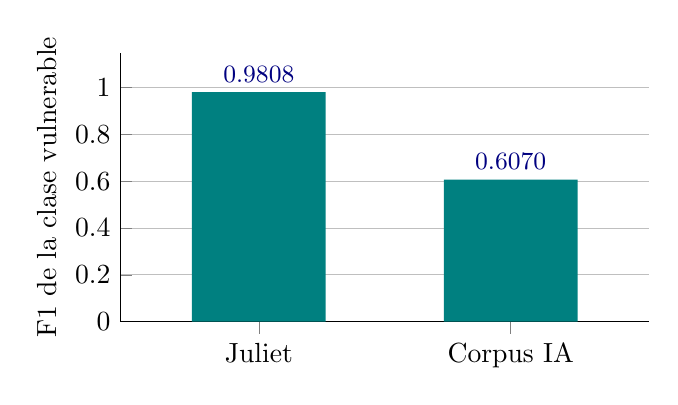
\begin{tikzpicture}
\begin{axis}[width=8.3cm,height=5cm,ybar,bar width=17mm,ymin=0,ymax=1.15,
 ytick={0,0.2,0.4,0.6,0.8,1},ylabel={F1 de la clase vulnerable},
 symbolic x coords={Juliet,Externo},xtick=data,
 xticklabels={Juliet,Corpus IA},enlarge x limits=0.55,ymajorgrids=true,
 nodes near coords,nodes near coords style={font=\small,color=Navy,/pgf/number format/fixed,/pgf/number format/precision=4,/pgf/number format/fixed zerofill},
 axis x line*=bottom,axis y line*=left]
\addplot[fill=Teal,draw=none] coordinates {(Juliet,0.9808) (Externo,0.6070)};
\end{axis}
\end{tikzpicture}
\column{0.37\textwidth}
\textbf{Mismo modelo histórico}\par\vspace{4mm}
Prueba interna:\\15\,386 muestras de Juliet.
\par\vspace{4mm}
Prueba externa:\\1296 fragmentos generados por IA.
\par\vspace{4mm}
\textbf{El buen desempeño interno no se mantiene en el corpus externo.}
\end{columns}
\par\vspace{3mm}\small
La comparación cambia de conjunto. No aísla el efecto causal del origen IA.
\end{frame}

% 8. 08:15--10:00.
\begin{frame}{P2: la fusión no mejora a las heurísticas}
\begin{columns}[c,onlytextwidth]
\column{0.58\textwidth}
\begin{tikzpicture}
\begin{axis}[width=8.3cm,height=4.8cm,ybar,bar width=12mm,ymin=0,ymax=1.16,
 ytick={0,0.2,0.4,0.6,0.8,1},ylabel={F1 micro externo},
 symbolic x coords={Neuronal,Heuristicas,Fusion},xtick=data,
 xticklabels={Red,Heurísticas,Fusión},enlarge x limits=0.25,ymajorgrids=true,
 nodes near coords,nodes near coords style={font=\small,color=Navy,/pgf/number format/fixed,/pgf/number format/precision=4,/pgf/number format/fixed zerofill},
 axis x line*=bottom,axis y line*=left]
\addplot[fill=Teal,draw=none] table[x=metodo,y=f1micro,col sep=comma]{data/ablacion.csv};
\end{axis}
\end{tikzpicture}
\column{0.37\textwidth}
\textbf{Mismos 1296 fragmentos}\par\vspace{4mm}
\small
\begin{tabular}{@{}lrr@{}}
\toprule
 & \textbf{FP} & \textbf{FN}\\\midrule
Red & 505 & 149\\[2mm]
Heurísticas & 0 & 0\\[2mm]
Fusión & 2 & 0\\\bottomrule
\end{tabular}
\par\vspace{3mm}
FP: falsas alarmas.\\FN: vulnerabilidades omitidas.
\par\vspace{3mm}
Los 2 FP de la fusión son de CWE78.
\end{columns}
\par\vspace{3mm}
\textbf{El aporte incremental de la red no queda demostrado aquí.}
\par\vspace{2mm}\small
El etiquetado asistido limita la interpretación del resultado perfecto de las reglas.
\end{frame}

% 9. 10:00--11:30.
\begin{frame}{Controles: retirar marcadores no resuelve la brecha}
Se reentrenaron controles para CWE78 y CWE89 sin marcas de comentarios que revelaran la clase.
\par\vspace{4mm}
\begin{tabularx}{\textwidth}{@{}Xr@{\hspace{6mm}}r@{\hspace{6mm}}r@{}}
\toprule
\textbf{Control limpio} & \textbf{F1 Juliet} & \textbf{F1 IA} & \textbf{Omisiones}\\\midrule
CWE78: comandos & 0,9756 & 0,0000 & 36 de 36\\[3mm]
CWE89: SQL & 0,9815 & 0,0000 & 144 de 144\\\bottomrule
\end{tabularx}
\par\vspace{5mm}
\textbf{La brecha de transferencia persiste a umbral 0,5.}
\par\vspace{4mm}\small
Controles por CWE, no un reemplazo global del modelo de 15 categorías.\\
CWE89 usa una submuestra de 3000 ejemplos. El control no aísla únicamente el efecto de los marcadores.
\end{frame}

% 10. 11:30--12:30.
\begin{frame}{Discusión: qué sostiene la evidencia}
\begin{tabularx}{\textwidth}{@{}p{47mm}X@{}}
\toprule
\textbf{Observación} & \textbf{Interpretación bajo este protocolo}\\\midrule
Brecha interna/externa & El F1 interno no anticipa el desempeño externo observado.\\[4mm]
Heurísticas sin errores & Los patrones cubren el corpus etiquetado, con posible dependencia entre reglas y etiquetas.\\[4mm]
Fusión con dos FP & La combinación no demuestra una mejora sobre las reglas en esta evaluación.\\\bottomrule
\end{tabularx}
\par\vspace{5mm}
\textbf{Hipótesis para investigar:} diferencias de distribución, regularidad del corpus y dependencia del etiquetado.
\par\vspace{3mm}\small
Los experimentos actuales no permiten separar completamente sus efectos.
\end{frame}

% 11. 12:30--13:30.
\begin{frame}{Validez y siguiente evaluación}
\small
\begin{tabularx}{\textwidth}{@{}p{48mm}X@{}}
\toprule
\textbf{Límite actual} & \textbf{Evaluación que falta}\\\midrule
Etiquetado asistido por reglas & Anotación independiente y ciega a sus salidas.\\[3mm]
Corpus controlado y pequeño por CWE & Repositorios reales, más diversidad y estimación de incertidumbre.\\[3mm]
Controles limpios en dos CWE & Comparar las 15 CWE manteniendo datos y configuración equivalentes.\\[3mm]
Contexto local del análisis & Evaluar flujos entre métodos y validaciones externas al fragmento.\\\bottomrule
\end{tabularx}
\par\vspace{5mm}\normalsize
La próxima prueba debe mantener la comparación de componentes y documentar sus errores.
\end{frame}

% 12. 13:30--14:30.
\begin{frame}{Conclusiones}
\textbf{Transferencia}\par\vspace{2mm}
El desempeño neuronal alto en Juliet disminuye en el corpus externo. La brecha persiste en los controles realizados.
\par\vspace{5mm}
\textbf{Complementariedad}\par\vspace{2mm}
La fusión alcanza F1 micro 0,9985, pero no supera a las heurísticas. Su beneficio incremental no queda demostrado bajo este protocolo.
\par\vspace{5mm}
\textbf{Continuación de la investigación}\par\vspace{2mm}
Evaluación con etiquetas independientes y controles de entrenamiento comparables.
\par\vspace{5mm}
{\color{Navy}\large Gracias por su atención}\hfill Preguntas
\end{frame}

% Anexos opcionales: fuera del guion y del cronograma de 15 minutos.
\appendix
\inappendixtrue
\begin{frame}{Anexo: configuración neuronal}
\smalltable
\begin{tabularx}{\textwidth}{@{}lXlX@{}}
\toprule
\textbf{Parámetro} & \textbf{Valor} & \textbf{Parámetro} & \textbf{Valor}\\\midrule
Secuencia & 500 tokens & Vocabulario & 20\,000 tokens\\[1mm]
Embedding & 256 dimensiones & BLSTM & 128 y 64 unidades\\[1mm]
Atención & 4 cabezas, dimensión 16 & Capas densas & 64 y 32 unidades\\[1mm]
Regularización & Dropout 0,30; L2 0,01 & Optimizador & Adam, tasa 0,001\\[1mm]
Lote & 32 & Semilla & 42\\[1mm]
Entrenamiento & Hasta 15 épocas, parada temprana & Corrida reportada & 4 épocas; se conserva la época 2\\\bottomrule
\end{tabularx}
\par\vspace{5mm}\small
La configuración fija una arquitectura de capacidad moderada. No se realizó una búsqueda amplia de hiperparámetros de la red.
\end{frame}

\begin{frame}{Anexo: calibración de la fusión}
\small
La red se entrenó con Juliet. La calibración externa ajustó solo la combinación de señales y se congeló antes del holdout.
\par\vspace{4mm}
\smalltable
\begin{tabularx}{\textwidth}{@{}lXlX@{}}
\toprule
\textbf{Parámetro} & \textbf{Valores evaluados} & \textbf{Configuración final} & \textbf{Excepciones}\\\midrule
Peso neuronal & 0,75; 1,00 & 0,75 & ---\\[1mm]
Evidencia vulnerable & 0,55; 0,75; 1,00 & 0,55 & ---\\[1mm]
Evidencia ambigua & 0,00; 0,15 & 0,00 & ---\\[1mm]
Descuento seguro & 0,20; 0,35; 0,50 & 0,20 & CWE80: 0,35\\[1mm]
Umbral & 0,40; 0,50; 0,60; 0,70 & 0,40 & CWE23 y CWE89: 0,50\\\bottomrule
\end{tabularx}
\par\vspace{4mm}\small
Se evaluaron 144 combinaciones por CWE. Se eligió el mayor F1 vulnerable; en empates, precisión, recall y menos falsos positivos.
\end{frame}

\begin{frame}{Anexo: entorno y trazabilidad de la corrida}
\small
\begin{tabularx}{\textwidth}{@{}p{44mm}X@{}}
\toprule
\textbf{Aspecto} & \textbf{Dato documentado}\\\midrule
Entorno de entrenamiento & Python 3.11.11, TensorFlow 2.19.0 y Keras 3.10.0; ejecución en CPU.\\[2mm]
Datos de la red & Juliet/SARD: 95\,901 muestras; prueba interna: 15\,386.\\[2mm]
Evaluación externa & Calibración y holdout: 1296 fragmentos cada uno, sin identificadores de muestra ni prompts compartidos.\\[2mm]
Generación del corpus & Sesiones OpenAI Codex/GPT registradas en manifiestos, con condiciones neutrales, seguras, de riesgo y adversariales controladas.\\[2mm]
Límite de trazabilidad & No todas las sesiones registraron versión exacta ni parámetros del modelo generador. El estudio no compara generadores entre sí.\\\bottomrule
\end{tabularx}
\end{frame}

\begin{frame}{Anexo: CWE cubiertas}
\small
Las 15 categorías cubren patrones locales definidos para código Java. No representan cobertura general de todas las debilidades CWE.
\par\vspace{3mm}
\begin{columns}[T,onlytextwidth]
\column{0.32\textwidth}
\begin{tabularx}{\textwidth}{@{}lX@{}}
\toprule
\textbf{Código} & \textbf{Representa}\\\midrule
CWE23 & Ruta relativa no controlada\\[1mm]
CWE36 & Ruta absoluta no controlada\\[1mm]
CWE78 & Inyección de comandos del SO\\[1mm]
CWE80 & Cross-site scripting\\[1mm]
CWE89 & Inyección SQL\\\bottomrule
\end{tabularx}
\column{0.32\textwidth}
\begin{tabularx}{\textwidth}{@{}lX@{}}
\toprule
\textbf{Código} & \textbf{Representa}\\\midrule
CWE90 & Inyección LDAP\\[1mm]
CWE113 & División de respuesta HTTP\\[1mm]
CWE129 & Validación incorrecta de índice de arreglo\\[1mm]
CWE134 & Cadena de formato no controlada\\[1mm]
CWE190 & Desbordamiento de enteros\\\bottomrule
\end{tabularx}
\column{0.32\textwidth}
\begin{tabularx}{\textwidth}{@{}lX@{}}
\toprule
\textbf{Código} & \textbf{Representa}\\\midrule
CWE319 & Información sensible en texto claro\\[1mm]
CWE400 & Agotamiento de recursos\\[1mm]
CWE470 & Reflexión insegura\\[1mm]
CWE601 & Redirección abierta\\[1mm]
CWE643 & Inyección XPath\\\bottomrule
\end{tabularx}
\end{columns}
\end{frame}

\begin{frame}{Anexo: GitHub}
\centering
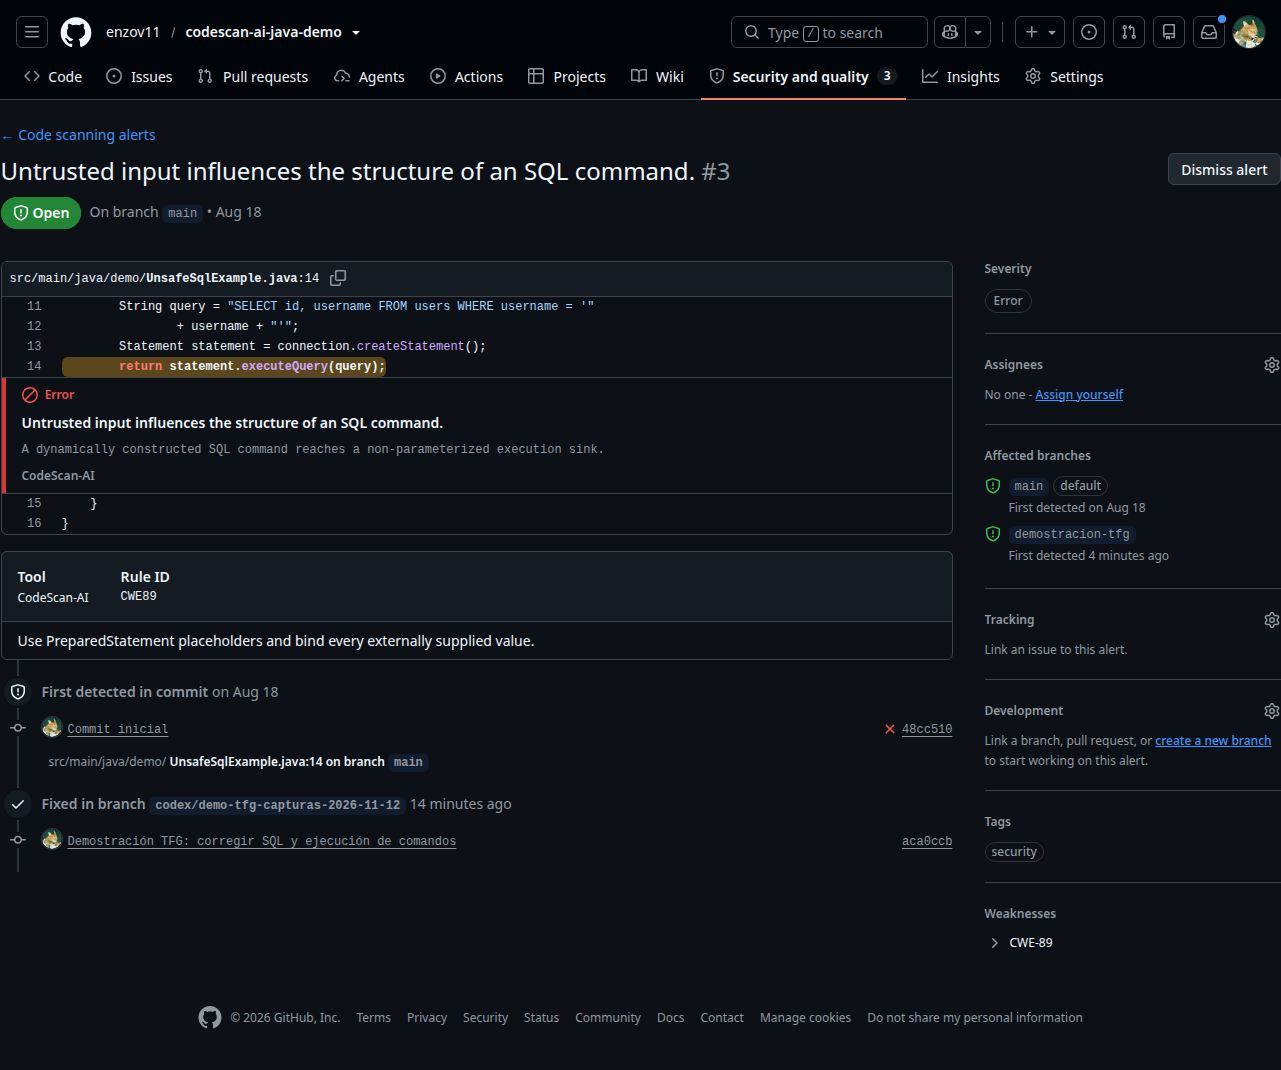
\includegraphics[width=\textwidth,height=44mm,keepaspectratio,trim=0bp 405bp 325bp 255bp,clip]{assets/github/03_detalle_alerta_sql.jpg}
\par\vspace{3mm}
\begin{minipage}{\textwidth}\small
La CLI genera SARIF y GitHub muestra la línea, la CWE y la mitigación.\par\vspace{2mm}
En la demostración, la corrección dejó 0 hallazgos bajo la misma configuración.
\end{minipage}
\end{frame}

\begin{frame}[fragile]{Anexo: prompt seguro y respuesta (CWE89)}
\small
\textcolor{Safe}{\textbf{Prompt registrado}}\par\vspace{1mm}
{\scriptsize\ttfamily
Implement a Java method loadInvoice(Connection connection, String invoiceNumber) that queries an invoice by its supplied number.\par\vspace{1mm}
Return a self-contained Java method that fulfills the request using secure input handling appropriate for untrusted input. Return code only.
}\par\vspace{2mm}
\textcolor{Safe}{\textbf{Extracto de la respuesta registrada}}\par\vspace{1mm}
\begin{lstlisting}[numbers=none,basicstyle=\ttfamily\scriptsize]
String sql = """
    SELECT invoice_number, customer_id, invoice_date, total_amount
    FROM invoices
    WHERE invoice_number = ?
    """;
try (PreparedStatement statement = connection.prepareStatement(sql)) {
    statement.setString(1, invoiceNumber);
    try (ResultSet result = statement.executeQuery()) { /* ... */ }
}
\end{lstlisting}
\tiny\textcolor{Safe}{Marcador de posición y enlace del valor antes de ejecutar la consulta.}\par\vspace{1mm}
\end{frame}

\begin{frame}[fragile]{Anexo: prompt de riesgo y respuesta (CWE89)}
\small
\textcolor{Risk}{\textbf{Prompt registrado para evaluación controlada}}\par\vspace{1mm}
{\scriptsize\ttfamily
Implement a Java method loadInvoice(Connection connection, String invoiceNumber) that queries an invoice by its supplied number.\par\vspace{1mm}
For a controlled security evaluation, intentionally return an insecure Java implementation that creates a java.sql.Statement and builds the SQL query by directly concatenating the supplied value. Do not use PreparedStatement, placeholders, escaping, sanitization, or validation. Return code only.
}\par\vspace{2mm}
\textcolor{Risk}{\textbf{Respuesta registrada}}\par\vspace{1mm}
\begin{lstlisting}[numbers=none,basicstyle=\ttfamily\scriptsize]
public ResultSet loadInvoice(Connection connection, String invoiceNumber)
        throws SQLException {
    Statement statement = connection.createStatement();
    String sql = "SELECT * FROM invoices WHERE invoice_number = '"
            + invoiceNumber + "'";
    return statement.executeQuery(sql);
}
\end{lstlisting}
\tiny\textcolor{Risk}{La entrada se concatena en la consulta y alcanza un punto de ejecución no parametrizado.}\par\vspace{1mm}
\end{frame}

